\begin{section}{Resultados}

A continuaci\'on, algunos resultados interesantes.

\begin{subsection}{Caso I}

Input: (AVIONES/BARCOS)

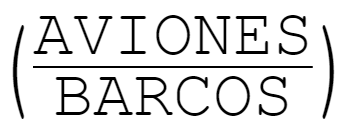
\includegraphics[scale=0.5]{./imgs/aviones.png}

La dificultad de este caso recae la divisi\'on de dos nodos no terminales (concatenaciones), donde la barra debe ajustarse al tama\~no del mayor de ellos y se debe centrar al menor. As\'i mismo, se deben ajustar los par\'entensis para abarcar toda la divisi\'on. 

\end{subsection}

\begin{subsection}{Caso II}

Input: MAR/(AGUA+SAL)

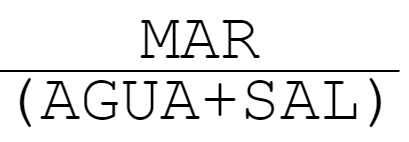
\includegraphics[scale=0.5]{./imgs/mar.png}

En esta oportunidad, la divisi\'on de, nuevamente, dos nodos no terminales (concatenaciones), con la diferencia de que los par\'entensis solo abarcan al denominador de la misma. Adem\'as, en este caso el numerador es aquel de longitud menor y por ende el que debe ser centrado.

\end{subsection}
\begin{subsection}{Caso III}

Input: VIENTO\^{}\{FUERTE\}/VELERO\_\{EN+PROBLEMAS\}

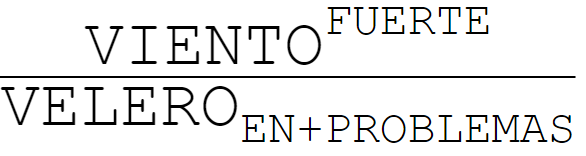
\includegraphics[scale=0.5]{./imgs/velero.png}

En este caso se incluyen sub\'indices y super\'indices, dentro de una divisi\'on, que es el nodo problem\'atico por excelencia.

\end{subsection}
\begin{subsection}{Caso IV}

Input: SUPER\^{}\{HEROE\}\_\{VILLANO\}


\includegraphics[scale=0.5]{./imgs/super.png}

La combinaci\'on de sub y super\'indices, ambos como concatenaciones encerradas por llaves para agruparlas.

\end{subsection}

\begin{subsection}{Caso V}

Input: (A\^{}BC\^{}D/E\^{}F\_G+H)-I

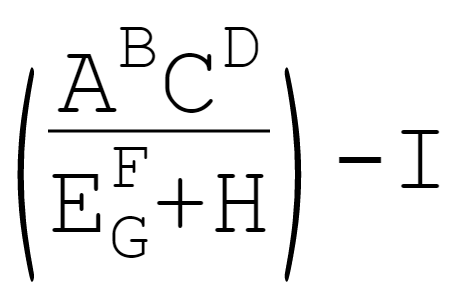
\includegraphics[scale=0.5]{./imgs/catedra.png}

Se expone el ejemplo de la c\'atedra, para luego aplicar una peque\~na modificaci\'on. Viendo que este ejemplo se visualiza bien, veamos de modificar el denominador, agregando una divisi\'on m\'as.

\end{subsection}

\begin{subsection}{Caso VI}

Input: (A\^{}BC\^{}D/E\^{}F\_G+\{H/J\})-I (ejemplo de la c\'atedra, versi\'on 2.0)

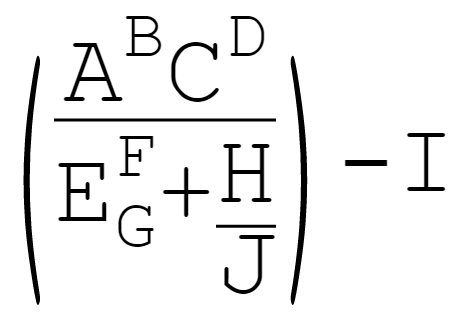
\includegraphics[scale=0.5]{./imgs/catedra2.png}

Por \'ultimo, se divide a H por J, consiguiendo que la concatenaci\'on no se rompa. Se puede apreciar que el tama\~no de la barra menor es el adecuado y est\'a bien situada, la H se desplaza hacia arriba unos mil\'imetros y los par\'entesis se alargan para abarcar la nueva divisi\'on. 

\end{subsection}
\end{section}
